






% \subsection{Angry Birds Levels}

\begin{figure}
\begin{center}
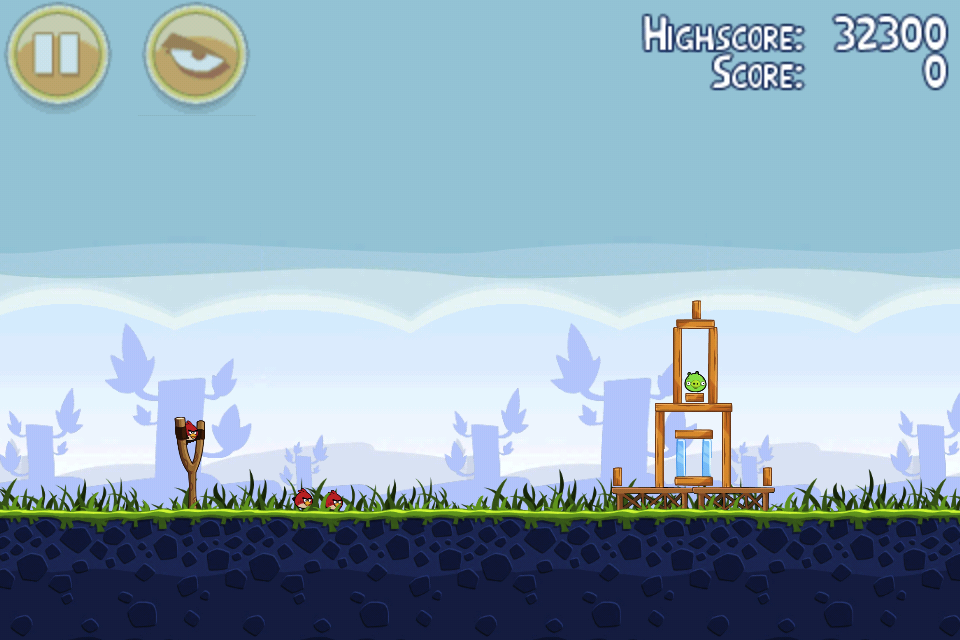
\includegraphics[trim = 0 100 0 150, clip, width=0.44\textwidth]{images/level.PNG}
\end{center}
\caption{Trivial Angry Birds level.}
\label{fig:easy-level}
\end{figure}

%The ultimate goal of Angry Birds is destroying pigs, but 
% [maybe cut this part]
The composition of each level can drastically affect the choice of strategy for playing the game. The player must reason with the available birds and their abilities, pigs, block structures, indestructible platforms, etc. Understanding these components of the game, as well as how they each affect the Angry Birds world and the outcome of the player's actions, is crucial to an effective strategy. 
Figure \ref{fig:easy-level} shows a simple level with red birds and a solitary pig protected by a weak structure. On the other hand, figure \ref{fig:hard-level} showcases a very difficult level where the only viable strategy for achieving a high score is executing precise shots which set off an explosive chain reaction. 


In this section, we will describe the composition of the levels and the various types of elements that require accurate modeling and understanding. 
\setlength{\belowcaptionskip}{-8pt}

\begin{figure}
\begin{center}
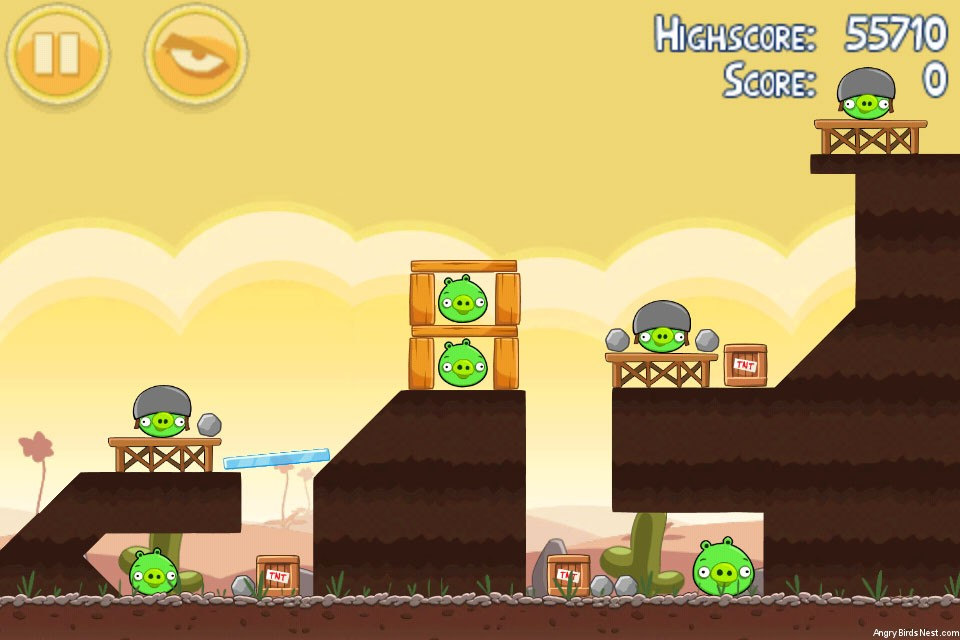
\includegraphics[trim = 0 20 0 20, clip, width=0.44\textwidth]{images/hard-level.jpg}
\end{center}
\caption{Difficult Angry Birds level.}
\label{fig:hard-level}
\end{figure}

% \subsubsection{Birds}
% Each level has an allotted number of birds that can be used by the player. The birds are launched from a slingshot and behave as expected under laws of motion and gravity. Each bird differs in their special ability which is activated by tapping on the screen while the bird is flying through the air, after being released from the slingshot and before hitting any objects. These special abilities of the birds are crucial to passing levels and achieving high scores, and thus need to be used strategically and accurately.

% \begin{figure}
% \begin{center}
% 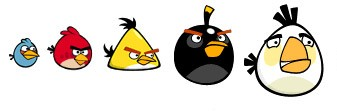
\includegraphics[trim = 0 10 0 10, clip, width=0.35\textwidth]{images/angry-birds-making-of-birds.jpg}
% \end{center}
% \caption{Basic birds available to the player in Angry Birds.}
% \label{fig:birds}
% \end{figure}

% \begin{itemize}
% \item \textbf{Red Bird} - no special powers.
% \item \textbf{Yellow Bird} - increases the velocity of the tapped bird.
% \item \textbf{Blue Bird} - splits into three birds on tap.
% \item \textbf{Black Bird} - Explodes on tap or after hitting an object.
% \item \textbf{White Bird} - drops an explosive egg on tap. 
% \end{itemize}


% \subsubsection{Pigs}
% The variety of birds is matched by the number of distinct pigs, however, the only difference between them is the amount of force needed to kill them. Pigs can be killed by a direct hit from a bird, or indirectly by falling blocks, explosions, or falls from heights. 

% \begin{figure}
% \begin{center}
% 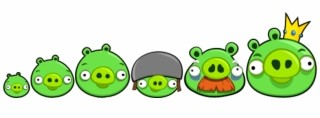
\includegraphics[trim = 0 20 0 20, clip, width=0.35\textwidth]{images/pigs.jpeg}
% \end{center}
% \caption{Basic pigs in Angry Birds.}
% \label{fig:pigs}
% \end{figure}

% \subsubsection{Blocks, Platforms, and Objects}
% Blocks are the fundamental elements that comprise each level. They come in various shapes, sizes, and materials, all of which impact how easily they can be destroyed or toppled over. Blocks made of ice break easily, stone blocks are harder to break, and wood blocks fit in between on this scale. TNT crates (shown in fig.~\ref{fig:hard-level} are a special block which explodes on impact, destroying close objects and launching others in the air. 
% On the other hand, platforms are indestructible floating objects which supplement the structural elements of Angry Birds. Together, the blocks and platforms are used to protect the pigs and force the player to opt for more elaborate strategy to win any given level. 

% \subsection{Viability as an AI Testbed}

% The Angry Birds scenario is an interesting testbed for AI, requiring a combination of multiple types of reasoning to effectively handle the game's full set of features. An intelligent agent playing Angry Birds needs to predict future states of the world that extend well beyond the immediate and direct consequences of the agent's actions. Each of the agent's actions often triggers a cascading chain of events causing drastic changes to the world. 

% The Angry Birds game is inherently a hybrid system, exhibiting both discrete and continuous behavior. A further complication is that Angry Birds contains non-linear dynamics which are difficult to handle. Furthermore, levels often contain a large number of objects, scaling up the size of the planning problem, while composite structures require a high level of abstract reasoning that AI agents are seldom capable of, further increasing the complexity of solving Angry Birds.

% Finally, Angry Birds derives a part of its complexity from the variety of its object types and their functionality. There is a wide range of distinct blocks which exhibit different features, and behave differently during interactions. A range of bird types, each with a distinct functionality which give the agent a large set of strategies to choose from when solving each individual level. 

% While the complexity of the full game can be at times overwhelming, Angry Birds provides a rich world for creating generalizable intelligent agents. That is, agents capable of reasoning about the long and short term consequences of their actions in continuous space and time with exogenous activity. All of the above points makes Angry Birds an important benchmark for the AI community and has driven researchers to create a clone of the game, called Science Birds\cite{renz2019ai}, for research purposes.






% Angry Birds is a well-known AI challenge problem. A scientific clone of the original game,Science Birds\cite{renz2019ai}, was recently developed to help researchers build better autonomous agents and perform controlled experiments. The game's simple layout and mechanics teamed with human players' innate spatio-temporal reasoning and forward state prediction makes for a compelling scenario for developing AI approaches. However, where humans excel, agents struggle. Minuscule errors in initial assumptions can result in scores and states drastically different from the player's predictions. Angry Birds requires a holistic understanding of each individual level and its relevant characteristics. Understanding the relevance of all features and the sum of all of its parts is not a common trait of AI approaches. Angry Birds is a difficult and fascinating challenge for autonomous agents, solving it would prove a significant milestone in Artificial Intelligence. 


Building an AI agent able to successfully play Angry Birds is an open challenge that requires reasoning about sequential actions in a continuous world with discrete exogenous events~\cite{renz2019ai}. 
Different versions of the game have proven to be NP-Hard, PSPACE-complete, and EXPTIME-hard~\cite{stephenson2020computational}, and the reigning world champion is still a human. 
% RONI: TEXT BELOW CAN BE OMITTED FOR SPACE
The game's simple layout and mechanics teamed with human players' innate spatio-temporal reasoning and forward state prediction makes for a challenging task. However, where humans excel, AI agents struggle. 
Minuscule errors in initial assumptions can result in scores and states drastically different from the player's predictions. Angry Birds requires a holistic understanding of each individual level and its relevant characteristics. Understanding the relevance of all features and the sum of all of its parts is not a common trait of AI approaches. Angry Birds is a difficult and fascinating challenge for autonomous agents, solving it would prove a significant milestone in Artificial Intelligence. 




% Our approach
Existing AI agents for this game are based on encoding domain-specific strategies and selecting from them~\cite{borovicka2014datalab,wang2017description}. 
In this work, we apply a domain-independent planner to solve this problem. 
Most existing domain-independent planning languages, such a STRIPS \cite{fikes1971strips}, PDDL \cite{mcdermott1998pddl}, and PDDL2.1 \cite{fox2003pddl2}, lack features to capture Angry Birds. 
Therefore, we modeled the problem using PDDL+ \cite{fox2006modelling}, which is a planning language that is designed for mixed discrete/continuous domains. PDDL+ enables reasoning about ballistic flight of birds and the consequences of their collisions with objects.

 


In this work, we make the following contributions: 
%(1) the first domain-independent approach for Angry Birds,[Roni: we can't saying  ``domain-independent approach for angry birds'' is a bit self-contradictory. I rephrased] 
(1) present the first successful application of domain-independent planning to solve Angry Birds,  (2) demonstrate its performance is on par with existing domain-specific approaches, 
(3) discuss the design choices around PDDL+ modeling needed to ensure computing solutions within timeouts. 


This work demonstrates that PDDL+ is useful for capturing challenging AI domains. 
However, an analysis of our performance show that solving planning problems in rich PDDL+ domains is a challenge for existing PDDL+ planners. The development of solutions for PDDL+ by the community has been slow. One of the reasons for this is that PDDL+ benchmark domains have been largely re-purposed from existing domains, which result in problems that could be addressed by PDDL2.1 techniques. 
%This leads to very few PDDL+ planners being developed and consequently little demand for PDDL+ domains. 
Thus, this work can serve as a call-to-arms for more research into PDDL+ planners and domain-independent heuristics. 


% Roni: Ideally say more about the design choices

The paper is organized as follows. We begin by providing an overview Angry Birds, and the Science Birds~\cite{renz2015aibirds} clone used for this research. This overview is followed by an analysis of different planning formalisms and their limitations for this domain. Next, we present the design of our PDDL+ domain for Angry Birds. We close with an evaluation of our approach on 100 Science Birds problems comparing our results with state-of-the-art baseline agents from previous competitions. %Roni: if space is an issue, this paragraph can be removed. It is not needed in a conference paper.

\section{Background: Angry Birds}
The objective in Angry Birds is to destroy pigs by launching birds at them from a slingshot. The pigs may be protected by structures built from blocks of various types. Each level of the game has an allotted number of birds that can be used, and pigs that need to be killed in order to pass the level. Destroying pigs and blocks earns the player points, as well as points for any unused birds after killing all pigs. 


% Angry Birds is a well-known AI challenge problem. A scientific clone of the original game,Science Birds\cite{renz2019ai}, was recently developed to help researchers build better autonomous agents and perform controlled experiments. The game's simple layout and mechanics teamed with human players' innate spatio-temporal reasoning and forward state prediction makes for a compelling scenario for developing AI approaches. However, where humans excel, agents struggle. Minuscule errors in initial assumptions can result in scores and states drastically different from the player's predictions. Angry Birds requires a holistic understanding of each individual level and its relevant characteristics. Understanding the relevance of all features and the sum of all of its parts is not a common trait of AI approaches. Angry Birds is a difficult and fascinating challenge for autonomous agents, solving it would prove a significant milestone in Artificial Intelligence. 

\subsection{Angry Birds Levels}

\begin{figure}
\begin{center}
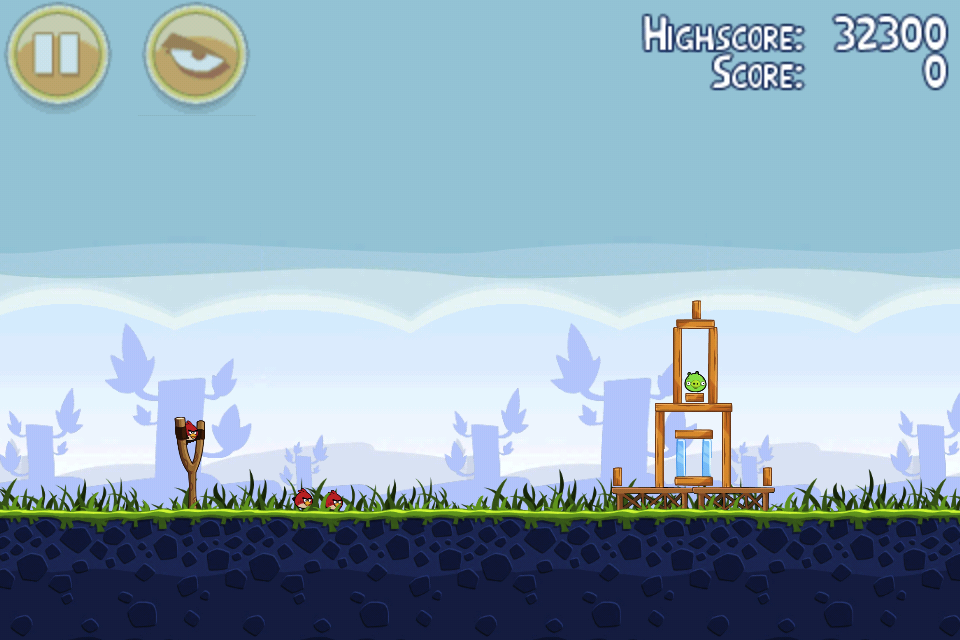
\includegraphics[trim = 0 100 0 150, clip, width=0.44\textwidth]{images/level.PNG}
\end{center}
\caption{Trivial Angry Birds level.}
\label{fig:easy-level}
\end{figure}

%The ultimate goal of Angry Birds is destroying pigs, but 
The composition of each level can drastically affect the choice of strategy for playing the game. The player must reason with the available birds and their abilities, pigs, block structures, indestructible platforms, etc. Understanding these components of the game, as well as how they each affect the Angry Birds world and the outcome of the player's actions, is crucial to an effective strategy. Figure \ref{fig:easy-level} shows a simple level with red birds and a solitary pig protected by a weak structure. On the other hand, figure \ref{fig:hard-level} showcases a very difficult level where the only viable strategy for achieving a high score is executing precise shots which set off an explosive chain reaction. In this section, we will describe the composition of the levels and the various types of elements that require accurate modeling and understanding. 

\setlength{\belowcaptionskip}{-8pt}

\begin{figure}
\begin{center}
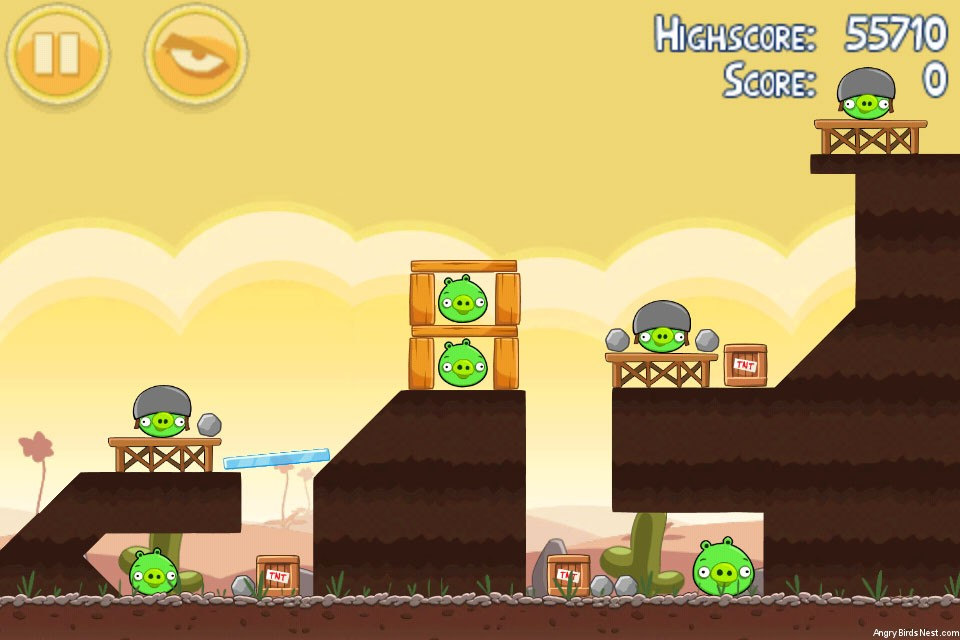
\includegraphics[trim = 0 20 0 20, clip, width=0.44\textwidth]{images/hard-level.jpg}
\end{center}
\caption{Difficult Angry Birds level.}
\label{fig:hard-level}
\end{figure}

\subsubsection{Birds}
Each level has an allotted number of birds that can be used by the player. The birds are launched from a slingshot and behave as expected under laws of motion and gravity. Each bird differs in their special ability which is activated by tapping on the screen while the bird is flying through the air, after being released from the slingshot and before hitting any objects. These special abilities of the birds are crucial to passing levels and achieving high scores, and thus need to be used strategically and accurately.

\begin{figure}
\begin{center}
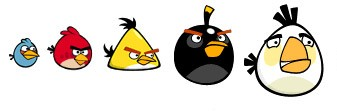
\includegraphics[trim = 0 10 0 10, clip, width=0.35\textwidth]{images/angry-birds-making-of-birds.jpg}
\end{center}
\caption{Basic birds available to the player in Angry Birds.}
\label{fig:birds}
\end{figure}

\begin{itemize}
\item \textbf{Red Bird} - no special powers.
\item \textbf{Yellow Bird} - increases the velocity of the tapped bird.
\item \textbf{Blue Bird} - splits into three birds on tap.
\item \textbf{Black Bird} - Explodes on tap or after hitting an object.
\item \textbf{White Bird} - drops an explosive egg on tap. 
\end{itemize}


\subsubsection{Pigs}
The variety of birds is matched by the number of distinct pigs, however, the only difference between them is the amount of force needed to kill them. Pigs can be killed by a direct hit from a bird, or indirectly by falling blocks, explosions, or falls from heights. 

\begin{figure}
\begin{center}
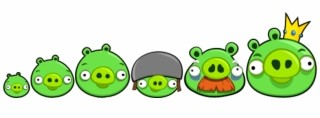
\includegraphics[trim = 0 20 0 20, clip, width=0.35\textwidth]{images/pigs.jpeg}
\end{center}
\caption{Basic pigs in Angry Birds.}
\label{fig:pigs}
\end{figure}

\subsubsection{Blocks, Platforms, and Objects}
Blocks are the fundamental elements that comprise each level. They come in various shapes, sizes, and materials, all of which impact how easily they can be destroyed or toppled over. Blocks made of ice break easily, stone blocks are harder to break, and wood blocks fit in between on this scale. TNT crates (shown in fig.~\ref{fig:hard-level} are a special block which explodes on impact, destroying close objects and launching others in the air. 
On the other hand, platforms are indestructible floating objects which supplement the structural elements of Angry Birds. Together, the blocks and platforms are used to protect the pigs and force the player to opt for more elaborate strategy to win any given level. 

\subsection{Viability as an AI Testbed}

The Angry Birds scenario is an interesting testbed for AI, requiring a combination of multiple types of reasoning to effectively handle the game's full set of features. An intelligent agent playing Angry Birds needs to predict future states of the world that extend well beyond the immediate and direct consequences of the agent's actions. Each of the agent's actions often triggers a cascading chain of events causing drastic changes to the world. 

The Angry Birds game is inherently a hybrid system, exhibiting both discrete and continuous behavior. A further complication is that Angry Birds contains non-linear dynamics which are difficult to handle. Furthermore, levels often contain a large number of objects, scaling up the size of the planning problem, while composite structures require a high level of abstract reasoning that AI agents are seldom capable of, further increasing the complexity of solving Angry Birds.

Finally, Angry Birds derives a part of its complexity from the variety of its object types and their functionality. There is a wide range of distinct blocks which exhibit different features, and behave differently during interactions. A range of bird types, each with a distinct functionality which give the agent a large set of strategies to choose from when solving each individual level. 

While the complexity of the full game can be at times overwhelming, Angry Birds provides a rich world for creating generalizable intelligent agents. That is, agents capable of reasoning about the long and short term consequences of their actions in continuous space and time with exogenous activity. All of the above points makes Angry Birds an important benchmark for the AI community and has driven researchers to create a clone of the game, called Science Birds\cite{renz2019ai}, for research purposes.




\section{Modeling Angry Birds}

In order to use a domain-independent planning approach, it is necessary to select a modeling language. Using the correct model representation language is crucial in ensuring efficiency, high performance, and accuracy in representing the structure and dynamics of the desired system. 

\subsubsection{Relevant Planning Languages}

Less expressive languages have been in use for decades and a multitude of efficient approaches have been developed over the years. Simple structure of the models and a limited set of features have allowed this area to concentrate on improving solvers and tackling large-scale problems. These languages are mostly propositional-only, and include STRIPS \cite{fikes1971strips}, ADL \cite{pednault1987formulating}, and PDDL \cite{mcdermott1998pddl}. However, such planning languages are unable to accurately represent real-world systems, only planning in restricted sub-problems and delegating reasoning to external solvers or semantic attachments.

%On the other hand, more expressive languages enable incorporating a rich set of features into the model without the need for external methods. 
One of the biggest leaps in expressiveness was made by the introduction of PDDL2.1~\cite{fox2003pddl2} which included support for numeric variables, explicit representation of time and durations, plan metrics, and continuous action effects (both linear and non-linear). It was quickly superseded by PDDL2.2~\cite{edelkamp2004pddl2} which encapsulates its predecessor's features (except continuous effects), and extended it by including timed-initial literals (TILs; unconditional events occurring at a pre-specified time in the plan) and derived predicates (propositional variables derived from \textit{if-then} rules rather than action). Both of these are powerful planning languages that standardized the modeling of important system features that edged AI planning closer to accurately representing real-world problems. However, the biggest gap between PDDL2.1/2.2 and realistic scenarios is the lack of support for modeling external influence. In Angry Birds, the agent needs to either utilize or mitigate the effects of activity beyond its control, such as gravity or explosions. In PDDL2.1, all change originates from the agent, whereas PDDL2.2 included only very-limited support for exogenous activity via derived predicates. 

PDDL, and its various versions, is accepted as the de facto standard planning language, though there have been attempts outside of it to define feature-rich models. One notable example is an extension to Functional STRIPS (FSTRIPS) described by \cite{ramirez2017numerical}. It allows modeling of hybrid systems but lacked full support for instantaneous exogenous activity, only able to define them as global constraints that invalidate the solution if triggered. However, in Angry Birds, there often exist cases where exogenous happenings have positive or neutral effects (w.r.t. finding a solution) and are a natural and integral part of the system (e.g. collisions). The FSTRIPS extension does not have the expressiveness to define such cases, and thus, it can only model a limited subset of hybrid systems accurately. 

\subsubsection{PDDL+}

To date, the language with, arguably, the most set of features relevant to real-world problems is PDDL+~\cite{fox2006modelling}. It was designed specifically as a planning standard for modeling hybrid systems (switched dynamical systems) governed by a set of differential equations and discrete mode switches. Formally defined as a mapping of planning constructs to Hybrid Automata~\cite{henzinger2000theory}, PDDL+ enables the modeling and solving of problems set in systems exhibiting both discrete mode switches and continuous flows. PDDL+ builds on the expressiveness of its predecessors, it encapsulates the entire set of features from PDDL2.1 (including continuous effects) and supplements that with the inclusion of timed-initial literals (TILs) from PDDL2.2. However, the biggest advancement over its predecessors is the inclusion of new constructs for defining exogenous activity in the domain.  

PDDL+ expresses exogenous activity using \textit{discrete events} and \textit{continuous processes}. Events represent the system's mode switches which instantaneously change the dynamics of the modeled system, whereas processes evolve the system over time dictated by a set of ordinary differential equations. Processes and events can be thought of as the world's version of durative and instantaneous actions, respectively. Exogenous activity is classed as 'must-happen' constructs, their effects are applied as soon as preconditions are satisfied. The agent can only interact with processes and events indirectly to mitigate or support their effects.

% \begin{figure}
% \begin{center}
% % \begingroup
%     \fontsize{8pt}{10pt}\selectfont
% \begin{verbatim}
%  (:event HIT-GROUND
%     :parameters (?b - ball)
%     :precondition (and
%         (not (held ?b))
%         (<= (distance-to-floor ?b) 0)
%         (> (velocity ?b) 0)  )
%     :effect (
%         (assign (velocity ?b) 
%             (* -0.8 (velocity ?b)))) )
% \end{verbatim}
% % \endgroup
% \caption{Example PDDL+ event modeling a ball bouncing off the ground.}
% \label{fig:event-pddl}
% \end{center}
% \end{figure}

% \begin{figure}
% \begin{center}
% % \begingroup
%     \fontsize{8pt}{10pt}\selectfont
% \begin{verbatim}
%  (:process FALLING
%     :parameters (?b - ball)
%     :precondition (and
%         (not (held ?b))
%         (< (velocity ?b) 100) )
%     :effect (and
%         (increase (velocity ?b) (* #t 9.8))
%         (decrease (distance-to-floor ?b) 
%                 (* #t (velocity ?b)))) )
% \end{verbatim}
% % \endgroup
% \caption{Example PDDL+ process modeling a falling ball.}
% \label{fig:process-pddl}
% \end{center}
% \end{figure}

The expressiveness of PDDL+ enables natural definitions of phenomena in Angry Birds. However, the resulting planning problems are notoriously difficult to solve due to immense search spaces and complex system dynamics. Indeed, planning in hybrid domains is challenging because, apart from the state space explosion caused by discrete state variables, the continuous variables cause the reachability problem to become undecidable~\cite{alur95algorithmic}. As a result, efficient model implementation is crucial to solving PDDL+ problems, arguably more so than for any other planing domain definition language. 


Recent works highlight how PDDL+ expressiveness teamed with clever system modeling can achieve high planning performance despite the problems' complexity in a range of domains, including Urban Traffic Control~\cite{vallati-et-al:aaai-2016}, Chemical Batch Plant~\cite{della2010pddl+}, Minecraft~\cite{roberts2017automated}, and Atmospheric Re-entry~\cite{piotrowski2018heuristics}). However, PDDL+ has been often misused. Indeed, even established hybrid domains are frequently only designed to test planner performance, instead of highlighting the complexity and importance of PDDL+ models. It is our belief that working in domains that require PDDL+, such as Science Birds, will foster the development of efficient planners to raise the prominence of PDDL+ planning. 
This will result in a virtuous cycle increasing the utility of PDDL+ in realistic applications. Next, we describe the contents and dynamics of the Angry Birds PDDL+ domain, highlighting how even complex and composite features can be efficiently encoded in the model and yield solvable problems. 

\subsection{PDDL+ Components of Angry Birds}

Angry Birds is a difficult scenario to define as a planning domain. It contains a variety of distinct object types and complex interweaving dynamics\footnote{Our Angry Birds PDDL+ model relies on knowledge obtained from Angry Birds where possible. Beyond parameters we could reliably source, we approximate the behavior and parameters to the best of our knowledge via experiments and observations.}. However, PDDL+ facilitates the modeling of such constructs and their implementation.

The objects in the Angry Birds domain are separated into four types: \textit{birds, pigs, blocks, and platforms}, each one is a crucial component of the game and requires explicit representation. Note that we did not list the slingshot, which is where the birds are launched from, as an object in the domain. 
Avoiding modeling unnecessary objects helps in maintaining a light-weight domain definition. 
So, instead of explicitly modeling the slingshot, we simply assign the coordinates of the at-rest slingshot to every bird that is about to be launched.

\noindent\textbf{Birds} The only objects directly controlled by the player are the birds. Each bird object requires a set of numeric functions to accurately track their state, including XY coordinates, velocities, mass, bounce count (denoting the number of times the bird collided with any other object), and an ID number to keep the order in which the birds are launched. This set of functions is supplemented by a single predicate for each bird stating whether it has been released from the slingshot. 

\noindent\textbf{Pigs} %Pigs are simply targets in our PDDL+ model, they 
A pig is represented by its XY position, radius, and mass functions, as well as a single predicate stating whether it is alive. Pigs are mostly static entities in Angry Birds and their PDDL+ representation is a straightforward translation.

\noindent\textbf{Blocks} The PDDL+ representation of blocks is very minimal. Each block is primarily defined by its basic characteristics, namely the XY coordinates, as well as the width and length values. Furthermore, blocks are also assigned values for mass, life-points, and stability (force needed to topple it), calculated based on the shape and size of the block, material (ice, wood, or stone), and what height it is positioned at (the taller a structure, the lower stability). Finally, each block is assigned a predicate dictating whether it is explosive to account for TNT crates. While there are different types of blocks in the Angry Birds game, we do not explicitly differentiate between them to keep the entire block ontology unified, and reduce unnecessary bloating of the domain. 

\noindent\textbf{Platforms} These Angry Birds elements are entirely static and indestructible, and modeled in PDDL+ via a pair of XY coordinates, supplemented by its width and height functions.

\smallskip
Finally, the model is supplemented by variables divided into two groups, global parameters and auxiliary operating parameters. The former includes important variables used globally in the system dynamics calculations, such as gravity, or launch angle and its rate of change. Auxiliary operating parameters are variables which play a supporting role such as denoting the currently active bird.

The number of predicates and functions per object type in the domain is purposely limited in numbers to facilitate efficient planning and maintain readability. This design decision was motivated by mitigating a lower planning performance in Angry Birds levels which often contain a multitude of distinct objects. As described above, each object is defined in PDDL+ by a set of state variables. Densely populated levels can cause states to drastically increase in size (often containing hundreds of variables each), which, in turn, can lead to significant drop in planner performance.

\subsection{PDDL+ Representation of Angry Birds Dynamics} 

The PDDL+ domain of Angry Birds features a variety of dynamics which dictate the change and evolution of the system. This however, creates planning problems with vast search spaces and large branching factors, making them computationally difficult to solve. Thus, mitigating the issues of solvability and efficiency was at the forefront of the domain's development at each step of the process, and is evident in the resulting PDDL+ model's composition.

\noindent\textbf{Actions} Angry Birds only features two types of actions from the player. %/agent. 
The first is launching a bird from the slingshot at a chosen angle, and the second is activating the special tap actions (if available). 

Launching of the bird is split into three separate phases: finding the angle, adjusting the launch velocity, and releasing the bird. This activity requires in-depth reasoning about the locations of the targeted structures, their strength and stability, and the force required to destroy or collapse them, in addition to the locations of pigs and other objects of interest (e.g. TNT crates). Encoding all of this information into actions would require complex constructs for each phase, and would result in concurrent and entangled behavior to account for both the angle and initial launch velocity. To mitigate the complexity of the launch action, we leverage the expressiveness of PDDL+ which allows us to delegate much of the activity away from the agent's control. 

First, we fix the launch velocity to its maximum possible value, removing the need for the agent deliberating over the power adjustment. This decision is motivated by the fact that maximum velocity shots are the most common as they provide widest range of targets and impact velocity is proportional to damage. This significantly simplifies the search phase and avoids the complexity associated with the interwoven nature of launch angle and velocity that the agent would have to otherwise reason with simultaneously. 

Next, we address the construction of the action responsible for selecting the launch angle. In a naive approach, one could encode a set of instantaneous actions which increase and decrease the angle, supplemented by an action releasing the bird from the slingshot.
%Another formalism that could be used to encode the launch action is to model it as a durative action with continuous effects (from PDDL2.1), increasing the angle over time.
However, leveraging the advantages of PDDL+ allows us to only require a single instantaneous action releasing the bird from the slingshot. We exploit the Theory of Waiting~\cite{mcdermott2003reasoning} which sees the agent idly waiting until the world evolves into a favorable state in which to execute actions. We pair the release action with a supporting process which continuously adjusts the angle as soon as a new bird is placed on the slingshot and is ready to be launched. This encoding reduces the number of decision points and the branching factor, mitigating state space explosion.

The effects of the release action (fig.~\ref{fig:action-pa-twang}) then assign values to the vertical and horizontal velocity variables based on the value of the angle. The velocities are then used to model the ballistic flight of the birds in the subsequent phase. Unfortunately, trigonometric functions are not included in PDDL+, thus our model relies on Bhaskara's and small-angle approximations for sine (\ref{eq:sin}) and cosine (\ref{eq:cos}), respectively (in the latter case, $\theta$ is expressed in radians). 
\begin{equation} \label{eq:sin}
\sin \theta \degree \approx \frac{4 \theta(180 - \theta)}{40500 - \theta(180 - \theta)}
\end{equation}
\begin{equation} \label{eq:cos}
\cos \theta \approx 1 - \frac{\theta^2}{2}
\end{equation}

% \setlength{\belowcaptionskip}{-15pt}

\begin{figure}
\begin{center}
% \begingroup
    \fontsize{8pt}{10pt}\selectfont
\begin{verbatim}
 (:action pa-twang
    :parameters (?b - bird)
    :precondition (and
        (= (active_bird) (bird_id ?b))
        (not (angle_adjusted))
        (not (bird_released ?b)) )
    :effect (and
        (assign (vy_bird ?b) 
            (* (v_bird ?b) SIN(angle)))
        (assign (vx_bird ?b) 
            (* (v_bird ?b) COS(angle)))
        (bird_released ?b)
        (angle_adjusted)) )
\end{verbatim}
% \endgroup
\caption{Action launching a bird (SIN and COS functions are approximated using eq.~\ref{eq:sin} \&~\ref{eq:cos}, respectively).}
\label{fig:action-pa-twang}
\end{center}
\end{figure}
\noindent As far as the birds' special actions are concerned, we defer their implementation to the next phase of our work. While most of their consequences are straightforward to implement, significant deliberation about their encoding is needed to maintain the model's efficiency. In the current version of the PDDL+ model, we only consider the basic behavior of birds without their special powers\footnote{While the tap actions are not yet implemented, in the Angry Birds environment where we execute our plans, the black bird's ability to explode is also triggered upon collision with any object after launch. At present, we keep the PDDL+ model oblivious to this ability, arguing that the model reflects the worst case scenario of launching an exploding bird. In practice, we notice that launching black birds yields higher returns in terms of points and destroyed targets than anticipated but does not perform worse than predicted during the planning phase.}. 

 The Angry Birds domain differs from more typical PDDL+ applications in that the vast majority of system dynamics is defined via exogenous activity and the agent's role is significantly diminished, simultaneously preserving the accuracy of the model and ensuring efficiency. 

\noindent\textbf{Processes}
The continuous behavior of Angry Birds is encapsulated using processes in the PDDL+ model. The first process is a linear increase in the current angle value, prior to launching a bird, based on a pre-defined rate of change (i.e. angle\_rate). The increase\_angle process (fig.~\ref{fig:process-launch}) is triggered as soon as the next bird in the queue is available for launch (i.e. at time-point t=0, or when the previously launched bird has expired). 


% \setlength{\belowcaptionskip}{-15pt}
\begin{figure}
\begin{center}
% \begingroup
    \fontsize{8pt}{10pt}\selectfont
\begin{verbatim}
 (:process increasing_angle
    :parameters (?b - bird)
    :precondition (and
        (not (angle_adjusted))
        (= (active_bird) (bird_id ?b))
        (not (bird_released ?b))
        (< (angle) (max_angle))
        (>= (angle) 0) )
    :effect (and
        (increase (angle) 
            (* #t (angle_rate)))) )
\end{verbatim}
% \endgroup
\caption{Process increasing the angle before launch.}
\label{fig:process-launch}
\end{center}
\end{figure}


Once the increase\_angle process terminates and the bird is launched, another process is triggered. The \textit{flying} process (fig.~\ref{fig:process-flying}) models ballistic flight of the active bird, updating it's velocity and location over time, according to the governing equations of motion. This is a crucial component of the system dynamics and the focal point of the whole Angry Birds domain, all of the post-launch environment changes must occur while this process is active. The flying process represents the domain's non-linear behavior, which is a major obstacle in PDDL+ planning as many planners struggle to handle complex dynamics. This situation is further complicated by the effects of multiple events which fire while the process is active and can drastically change its behavior with each triggered activity. Crucially, this process could not be encoded using the predecessors of PDDL+ as they either cannot accurately represent the system dynamics or require the agent's command to begin and end continuous activity. 

% \setlength{\belowcaptionskip}{-15pt}
\begin{figure}
\begin{center}
% \begingroup
    \fontsize{8pt}{10pt}\selectfont
\begin{verbatim}
 (:process flying
    :parameters (?b - bird)
    :precondition (and
        (bird_released ?b)
        (= (active_bird) (bird_id ?b))
        (> (y_bird ?b) 0) )
    :effect (and
        (decrease (vy_bird ?b) 
            (* #t (gravity) ))
        (increase (y_bird ?b) 
            (* #t (vy_bird ?b)))
        (increase (x_bird ?b) 
            (* #t (vx_bird ?b)))) )
\end{verbatim}
% \endgroup
\caption{PDDL+ process of a bird's flight.}
\label{fig:process-flying}
\end{center}
\end{figure}
\noindent\textbf{Events} 
%In the grand scheme of our Angry Birds model composition, 
The vast majority of the Angry Birds system mechanics are event-driven. Each object in the game has one or more associated events which govern their interactions with the environment and other objects in the level. They enable modeling of complex behavior including all collisions, destructions, explosions, and structure collapses. Events are also modeling supporting features such as loading the next bird into the slingshot or expiring the currently active bird. Finally, events are the only means of achieving planning goals, and, in fact, all of the post-launch system dynamics are caused by events interacting with the effects of the flying process. 

Collisions are the first class of events that are highlighted in an Angry Birds problem. The main aim of the game is to kill pigs by either directly colliding with them, or destroying blocks such that pigs are killed by collapsing structures, falling from heights, or causing nearby explosions. Each of those cases is a crucial tactic in Angry Birds, and all accurate models of the game need to represent such mechanics. 

Direct interactions between a bird and a pig are modeled based on elastic sphere collisions in two dimensions. Pigs are extremely fragile and thus disappear upon almost any contact from another object. Thus after a collision, only the bird's resulting velocity needs to be calculated, according to the angle-free elastic collision formula:
\begin{equation} \label{eq:collision}
\vec{v}_{b}' = \vec{v}_{b} - \frac{2m_{p}}{m_{b}+m_{p}} \frac{\langle \vec{v}_{b} - \vec{v}_{p},\vec{x}_{b} - \vec{x}_{p}\rangle}{||\vec{x}_{b} - \vec{x}_{p}||^2}(\vec{x}_{b} - \vec{x}_{p})
\end{equation}
where $\vec{v}_b$ and $\vec{v}_p$ are the velocity of the bird and pig, respectively, $\vec{x}_b$ and $\vec{x}_p$ are their respective positions, $m_b$ and $m_p$ are their respective masses, and the angle brackets denote an inner product of two vectors. 
Translating this equation into a PDDL+ event allows us to model behavior beyond the obvious solutions. Indeed, it enables the planner to find highly innovative solutions such as deliberately and directly killing two pigs with one bird (fig.~\ref{fig:double-hit}).

The ground in Angry Birds is often overlooked when playing the game but it can prove useful when aiming at difficult targets. As such, an event (seen in fig~\ref{fig:ground-event} is defined in the domain that influences the bird's trajectory after bouncing off the ground, based on energy lost during the collision (i.e. ground damper). Figure~\ref{fig:bounce-hit} shows how a ground-bounce event helps in killing a pig when a direct hit is impossible.
% \setlength{\belowcaptionskip}{-10pt}
\begin{figure*}
\begin{center}
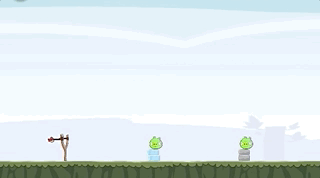
\includegraphics[width=0.23\textwidth]{images/double1.png}
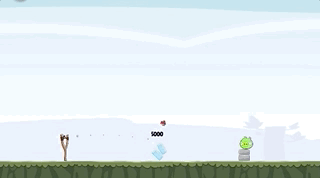
\includegraphics[width=0.23\textwidth]{images/double2.png}
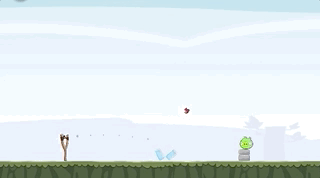
\includegraphics[width=0.23\textwidth]{images/double3.png}
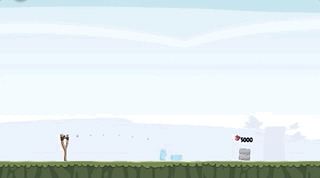
\includegraphics[width=0.23\textwidth]{images/double4.png}
\end{center}
\caption{Two pigs-one bird plan in execution.}
\label{fig:double-hit}
\end{figure*}

\begin{figure*}
\begin{center}
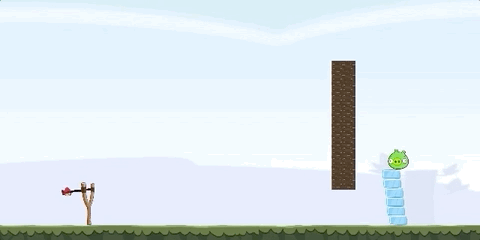
\includegraphics[width=0.23\textwidth]{images/under1.png}
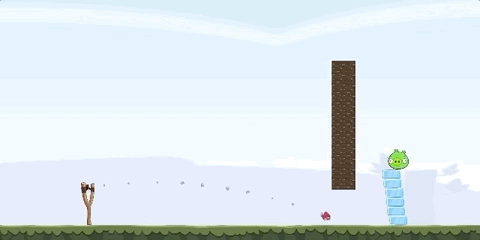
\includegraphics[width=0.23\textwidth]{images/under2.png}
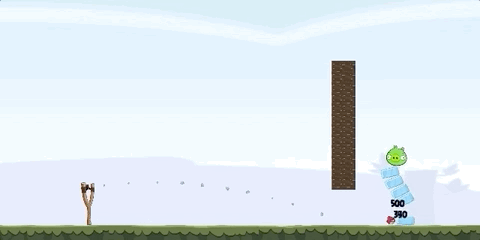
\includegraphics[width=0.23\textwidth]{images/under3.png}
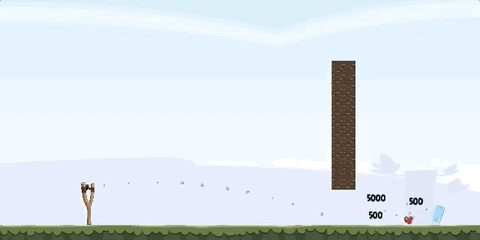
\includegraphics[width=0.23\textwidth]{images/under4.png}
\end{center}
\caption{Solution requiring bouncing of the ground and collapsing a structure to kill the target pig.}
\label{fig:bounce-hit}
\end{figure*}

\setlength{\belowcaptionskip}{0pt}
\begin{figure}[!ht]
\begin{center}
% \begingroup
    \fontsize{8pt}{10pt}\selectfont
\begin{verbatim}
(:event collision_ground
  :parameters (?b - bird)
  :precondition (and
    (= (active_bird) (bird_id ?b))
    (<= (y_bird ?b) 0)  )
  :effect (and
    (assign (y_bird ?b) 1)
    (assign (vy_bird ?b) 
    (* (* (vy_bird ?b) -1)(ground_damper)))
    (assign (bounce_count ?b) 
    (+ (bounce_count ?b) 1))) )
\end{verbatim}
% \endgroup
\caption{Event modeling a bird bouncing off the ground.}
\label{fig:ground-event}
\end{center}
\end{figure}

\smallskip
Most interactions in a level occurs between birds and blocks in the scene. Blocks form structures which act as a protection barrier for targeted pigs. Thus, modeling collisions with blocks is vital to an accurate representation of Angry Birds. However, similarly to pig collisions, we opt to only define the event's effects in terms of the impact it has on the bird's velocity and the blocks stability and life values. There are two separate events modeling bird-block collisions with the distinction based on whether the block is stable enough to withstand the impact without being knocked out of place or destroyed entirely. In such cases, the bird bounces back off the block, otherwise it continues moving forward though with a diminished velocity. 

We decided that modeling the motion of blocks after impact, and chains of block-block collisions, using continuous dynamics would be prohibitively difficult. Such endeavor would require a significant implementation effort, defining a process for tracking each individual block's change in position and rotation over time, as well as a set of events to account for secondary interactions. These additions would only marginally improve the domain's accuracy, though the planner would experience a drastic drop in performance, having to keep track of dozens of simultaneous non-linear processes in every state after a collision.

An additional event is present in the domain to account for a special case of block-block interactions, namely dislodging or destroying blocks supporting larger structures. In such cases, an event is triggered for every supported block, reducing its stability value to 0, repositioning the block to the ground, and adjusting its life value to account for fall damage. Analogously, we defined another event for killing pigs which sit atop of collapsing block structures. Figure~\ref{fig:bounce-hit} showcases the execution of a plan which includes a ground-bounce event, followed by the collapse of a tall structure to kill an otherwise unreachable target pig.

The two final block-related events concern exploding TNT crates. Any impact upon the crate causes an explosion destroying all objects in its immediate vicinity and displacing objects further away. In our PDDL+ model, we incorporate two simple events modeling the explosive destruction of pigs and blocks nearby a TNT crate. As previously indicated, we omit the movement of objects caused by the explosion. 

The described events account for a significant portion of interactions during gameplay where birds are used to destroy multi-block structures to expose or kill targeted pigs, when a direct hit is infeasible or impossible.

Platforms are indestructible objects which the agent needs to reason with to avoid poor results. However, almost no meaningful interactions occur between birds and platforms, and thus our domain contains an event modeling this type of collision but only to discourage the agent from shooting at platforms. The event deters the agent by nullifying the bird's velocity and expiring it without any impact on the level.

Finally, we encode a supporting event which models the end of life for an active bird. In the game, a bird expires when it moves beyond the limits of the scene or when it stops moving. Modeling the exact timing of the end of a birds life is quite difficult. Instead, we define the birds usefulness in terms of the number of bounces off other objects. Each bounce partially reduces the bird's momentum, and its collision impact becomes negligible after three bounces. Therefore, we define a termination event for the active bird once it has bounced three times. The result of this event is that the next bird can be placed on the slingshot for launch.

\textbf{Goals}
While the goal of Angry Birds is to destroy all of the pigs, we consider different formulations for individual planning problems. First, the full planning problem uses the goal of destroying all of the pigs, and considers all available birds. Second, a simplified problem splits the original scenario into single-bird episodes with the goal of killing at least one pig. Third, the relaxed simplified problem also reasons with single-bird episodes, but only considers platforms and pigs, ignoring all other objects. In the experiment below, we start with the simplified approach and use the relaxed simplified version of the problem as a contingency strategy when the first planning phase fails to find a solution.

\setlength{\belowcaptionskip}{-10pt}
\begin{table}[h]
\centering
\scriptsize
\resizebox{\columnwidth}{!}{%
\begin{tabular}{c|c|c|c|c|}
\cline{2-5}
 & \textbf{PDDL+} & \textbf{PDDL2.1} & \textbf{PDDL2.2} & \textbf{FSTRIPS+} \\ \hline
\multicolumn{1}{|c|}{Bird Flight}              & $\checkmark$ & $\circ$ &  & $\checkmark$ \\ \hline
\multicolumn{1}{|c|}{Collisions}               & $\checkmark$ &   & $\checkmark$   & \\ \hline
\multicolumn{1}{|c|}{Explosions}               & $\checkmark$ &   & $\checkmark$   & \\ \hline
\multicolumn{1}{|c|}{Structure collapse}       & $\checkmark$ &   & $\checkmark$   & \\ \hline
\end{tabular}%
}
\caption{Language support for crucial Angry Birds features.}
\label{tab:lang-comparison}
\end{table}

\smallskip
To further solidify out choice of PDDL+ for modeling Angry Birds, table~\ref{tab:lang-comparison} shows an overview of relevant languages' ability to model crucial features of Angry Birds (note that PDDL2.1 can model the non-linear dynamics of flight but only as a durative action). As can be seen, only PDDL+ has the capacity to model and reason with all elements and dynamics of the game. Understanding the challenges of planning with such feature-rich models enabled us to make informed design decisions and preemptively mitigate any risks associated with PDDL+.



\section{Experiments}

The yearly Angry Birds competition~\cite{renz2015aibirds} at IJCAI ran by researchers from ANU yielded a number of game-playing AI agents. In this section, we compare our PDDL+ planing approach (named HYDRA) to solving Angry Birds against 3 different agents:

\begin{itemize}
    \item \textbf{DataLab}~\cite{borovicka2014datalab} is the 2014 \& 2015 champion developed by researchers from Czech Technical University. The agent's actions are based on predicted utility of pre-defined strategies (destroy pigs, target TNT, target round blocks, destroy structures).
    \item \textbf{Eagle's Wing}~\cite{wang2017description} is a triple champion (2016-18) developed by University of Waterloo. Eagle's Wing selects from 5 predefined strategies (pigshooter, TNT, most blocks, high round objects, and bottom building blocks), based on predicted utility. Eagle's Wing supplements these strategies with a trained xgbost model to optimize its performance.
    \item \textbf{Naive Agent}~\cite{stephenson2017creating} was developed by ANU as a baseline for the competition. It targets a randomly selected pig with each active bird, and has predefined windows for tap actions per bird type. The Naive agent only considers the locations of visible pigs, disregarding all other objects in the scene.
\end{itemize}

We conduct the experiments using the ANU Science Birds framework as all agents have been developed to work with its API. The API provides the ground truth as a list of labeled objects and their locations. Our agent supplements the ground truth information with our own deduced knowledge of the game and its objects. These are then merged and automatically translated into a PDDL+ problem file, encoding the collective relevant information about each level. Using a 30s timeout, we first attempt to generate plans using the simplified planning problem. If no plan is found in 30s, we use the relaxed simplified problem. If again, no plan is found, we execute a default non-planning action.

The choice of PDDL+ planner for our agent was motivated by the capabilities and performance of available software. The Angry Birds domain requires a high-performing planner able to handle large numbers of happenings, wide range of model features, and non-linear system dynamics.

SMTPlan+~\cite{cashmore2016compilation} is a recent planner able to reason with all features of PDDL+ but it is only capable of dealing with polynomial non-linearity and does not scale well with the number of happenings. UPMurphi~\cite{della2009upmurphi} is a highly optimized PDDL+ planner which solves hybrid planning problems via a uniform discretization approach. UPMurphi can reason with the entire set of PDDL+ features and non-linear dynamics, though it is limited in performance by lack of heuristics. DiNo~\cite{piotrowski2016heuristic} is a PDDL+ planner which builds on the strengths of UPMurphi and extends it by implementing a domain-independent heuristic. However, DiNo's heuristic is computationally expensive and does not perform well on the Angry Birds domain, defeating its purpose. ENHSP~\cite{scala2016interval} is a planner for numeric domains equipped with an efficient heuristic. However, it can only handle problems encoded using the hybrid systems extension of FSTRIPS language which, as described before, is insufficiently expressive to model the Angry Birds domain. With that in mind, we concluded that UPMurphi was the best available planner and chose it for our evaluation.

% \setlength{\belowcaptionskip}{-12pt}

\begin{table}[ht!]
\centering
\small
\begin{tabular}{|c|c|c|}
\hline
\textbf{Agent} & \textbf{Problems Solved} & \textbf{Avg. Score per Level} \\ \hline
Naive (ANU)    & \textbf{49}              & 45,112.4                      \\ \hline
HYDRA          & 44                       & \textbf{47,515.7}             \\ \hline
DataLab        & 26                       & 46667.8                      \\ \hline
Eagle's  Wing  & 16                       & 39152.0                      \\ \hline
\end{tabular}
\caption{Evaluation results (solved levels and avg. scores).}
\label{tab:results}
\end{table}

\subsection{Evaluation Results}

For the evaluation, each agent attempted to solve a set of 100 random Angry Birds levels, developed using ANU's level generator\footnote{We used existing levels generated by ANU, which can be found at~\url{https://gitlab.com/aibirds/sciencebirdsframework/}}. As can be seen from the overall results (Tab.\ref{tab:results}), the Naive agent performed best overall solving 49 problems, followed closely by our HYDRA approach on 44 problems solved. Surprisingly, both Datalab and Eagle's Wing agents significantly underperformed on the evaluation test set, solving 26 and 16 problems, respectively. Fig.~\ref{fig:scores-plot} plots each agent's scores for each level in the evaluation, for readability purposes we sorted the level ordering (x axis) by HYDRA scores. The HYDRA agent performs best in terms of point scored, achieving an average score of 47515.7 points per level. Surprisingly, Datalab achieved an average score of 46667.8, outscoring the Naive agent (45112.4 points), even though the former solves significantly fewer levels. These results support the claim that our domain-independent planning approach is on par with existing domain-dependent approaches, even without encoding the birds' special powers.

\setlength{\belowcaptionskip}{-5pt}

\begin{figure}[htbp!]
\begin{center}
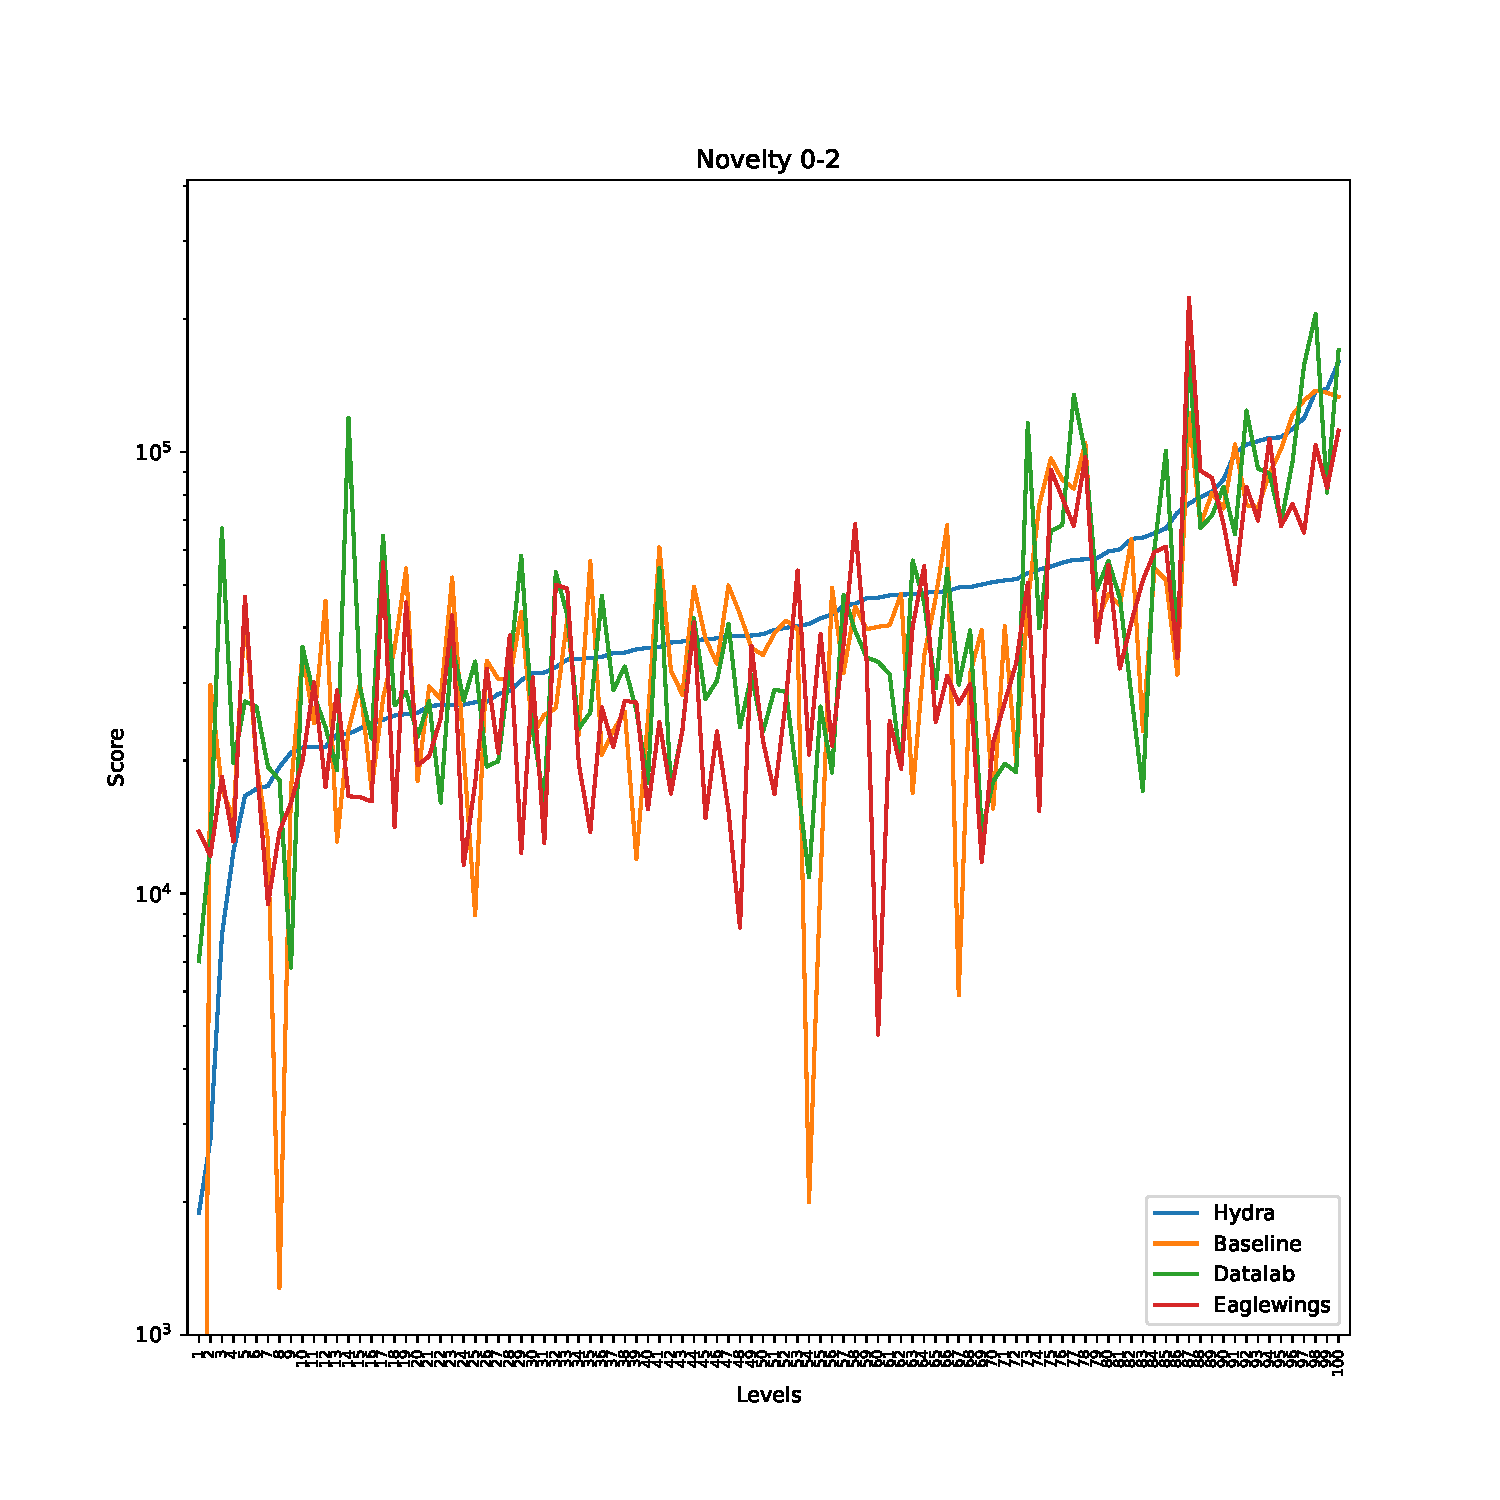
\includegraphics[trim= 50 45 50 82, clip, width=0.44\textwidth]{images/plot_novelty0_log.pdf}
\end{center}
\caption{Points per level (sorted by HYDRA scores).}
\label{fig:scores-plot}
\end{figure}

The speculative cause for Eagle's Wing and DataLab's low performance might be attributed to the fact that the AI competition tested on hand-designed Angry Birds levels with specific winning strategies devised by their creators. Both agents rely on human devised strategies which proved to work well on the original Angry Birds levels but struggle to solve levels created by an automated generator, lacking depth to effectively reason with level composition. 

To determine if computational resources played a significant role in our performance, we report the number of shots performed as a result of different planning problems. Out of 358 possible shots in the evaluation only 34 used the relaxed simplification, and 30 employed the default non-planning action strategy. This indicates that one could improve performance through either a more accurate PDDL+ encoding of Angry Birds, or PDDL+ planner heuristics to tackle the full goal planning problems. We intend to pursue both courses of action in future phases of our research.

One observation from the evaluation is that ANU's level generator produces compositions that rarely require advanced reasoning about the level's structure. Many of the generated levels can be  solved by only targeting pigs, as proved by the results of our experiments where the Naive agent outperformed sophisticated strategies of Eagle's Wing and Datalab. In future experiments we will aim to compose a set of test levels which require more diverse reasoning and strategies to achieve high scores.

\section{Conclusion}

We presented a novel PDDL+ planning model of Angry Birds, one of the most popular mobile games and a challenging AI testbed. It requires a highly expressive modeling language to capture  dynamics of the system. We determined the best way to accurately modeling the game as a planning domain is with PDDL+, an advanced planning language developed for hybrid systems. PDDL+ introduced a standardized method for including exogenous activity in planning domains via discrete events and continuous processes, which are critical to modeling Angry Birds' fundamental features. Next, we showed how leveraging the expressiveness of PDDL+ can mitigate its inherent risks and complexity while maintaining planning efficiency. Our evaluation showed promising results, with our agent (HYDRA) reaching the overall highest average score per level and significantly outperforming multiple champions of the Angry Birds AI competition. 

By representing Angry Birds as a planning domain, we have proved that PDDL+ is capable of modeling a challenging AI problem. We argue that PDDL+ is currently severely underused due to modeling complexity and large search spaces. However, we have shown that the expressiveness of PDDL+, in fact, facilitates building of efficient models which can mitigate these issues and enable solving of interesting and important problems. We plan on further extending our domain to improve its accuracy. Simultaneously, we aim to develop domain-independent heuristics for more efficient PDDL+ planning.


\newpage
